\documentclass[11pt]{article}
\usepackage[margin=1in]{geometry}
\usepackage[T1]{fontenc}
\usepackage{lmodern}
\usepackage{amssymb}
\usepackage{graphicx}
\usepackage{float}
\usepackage{adjustbox}
\usepackage[font=small,labelfont=bf]{caption}
\usepackage[authoryear,round]{natbib}
\usepackage{xurl}
\usepackage[colorlinks=true,linkcolor=blue,citecolor=blue,urlcolor=blue]{hyperref}

% ---- Edit this ---------------------------------------------------------------
\newcommand{\replicationURL}{https://github.com/USERNAME/REPO}  % repository link
% -------------------------------------------------------------------------------

% Paths are relative to this file (paper/). Figures and tables are written by the
% R scripts in code/ into output/.
\graphicspath{{../output/figures/}}
% \tab{file}: input a stargazer table, shrinking it to the text width if needed
\newcommand{\tab}[1]{{%
  \let\origtabular\tabular \let\endorigtabular\endtabular
  \renewenvironment{tabular}{\begin{adjustbox}{max width=\textwidth}\origtabular}{\endorigtabular\end{adjustbox}}%
  \input{../output/tables/#1}}}

\title{PLSC 508 Replication and Extension:\\ Network, Vertex Attributes, and Reproduction}
\author{Yasin Shafi}
\date{\today}

\begin{document}
\sloppy
\maketitle

\section*{Study and Repository}

\noindent Study reproduced: \citet{right2025pushing}. Pushing Back or Backing Down? Evidence on Donor
Responses to Restrictive NGO Legislation. \textit{International Organization} 79(4): 759--786.
\href{https://doi.org/10.1017/S0020818325100957}{doi:10.1017/S0020818325100957}.

\medskip
\noindent Repository (data, R code for every result in this document, and \texttt{README.txt}):
\url{\replicationURL}.
The authors' original files are on Harvard Dataverse \citep{right2025replication},
\href{https://doi.org/10.7910/DVN/FIINC8}{doi:10.7910/DVN/FIINC8}.

%===============================================================================
\section{The Network}

The original study is a dyadic panel analysis, not a network analysis. The extension
treats the same data as a sequence of yearly two-mode (bipartite) networks, 2005--2019
(\texttt{code/02\_build\_network.R}).

\begin{itemize}
  \item \textbf{Nodes, mode 1 (donors):} the 19 large OECD DAC donors in the original study.
  \item \textbf{Nodes, mode 2 (recipients):} aid-receiving countries in the original analysis
        sample, 105--109 per year. As in the paper, countries with population below 2 million
        in every year are excluded.
  \item \textbf{Ties:} donor $i$ is tied to recipient $j$ in year $t$ if $i$'s democracy-aid
        commitment to $j$ in $t$ is positive (OECD CRS commitments, the paper's democracy-sector
        coding). The commitment amount (USD) is stored as an edge attribute. A parallel
        economic-aid network uses economic-sector commitments.
  \item \textbf{Structure:} ties run only between modes. There are no donor--donor or
        recipient--recipient ties. The data are a balanced donor $\times$ recipient panel, so
        an absent tie is an observed zero, not missing data.
\end{itemize}

Donor--donor ``co-funding'' ties (two donors funding the same recipient) would come from a
one-mode projection of this bipartite network. A projection discards information and
mechanically creates clustering. Projections are therefore used only descriptively; the
extension models the bipartite network directly. Table~\ref{tab:netdesc} reports size and
density by year. Both networks are dense: about 60\% of possible democracy-aid ties and
80\% of possible economic-aid ties are present. The extension will test whether results
depend on the ``any positive commitment'' tie definition by using higher thresholds.

\tab{tab_network_desc.tex}

\begin{figure}[H]
  \centering
  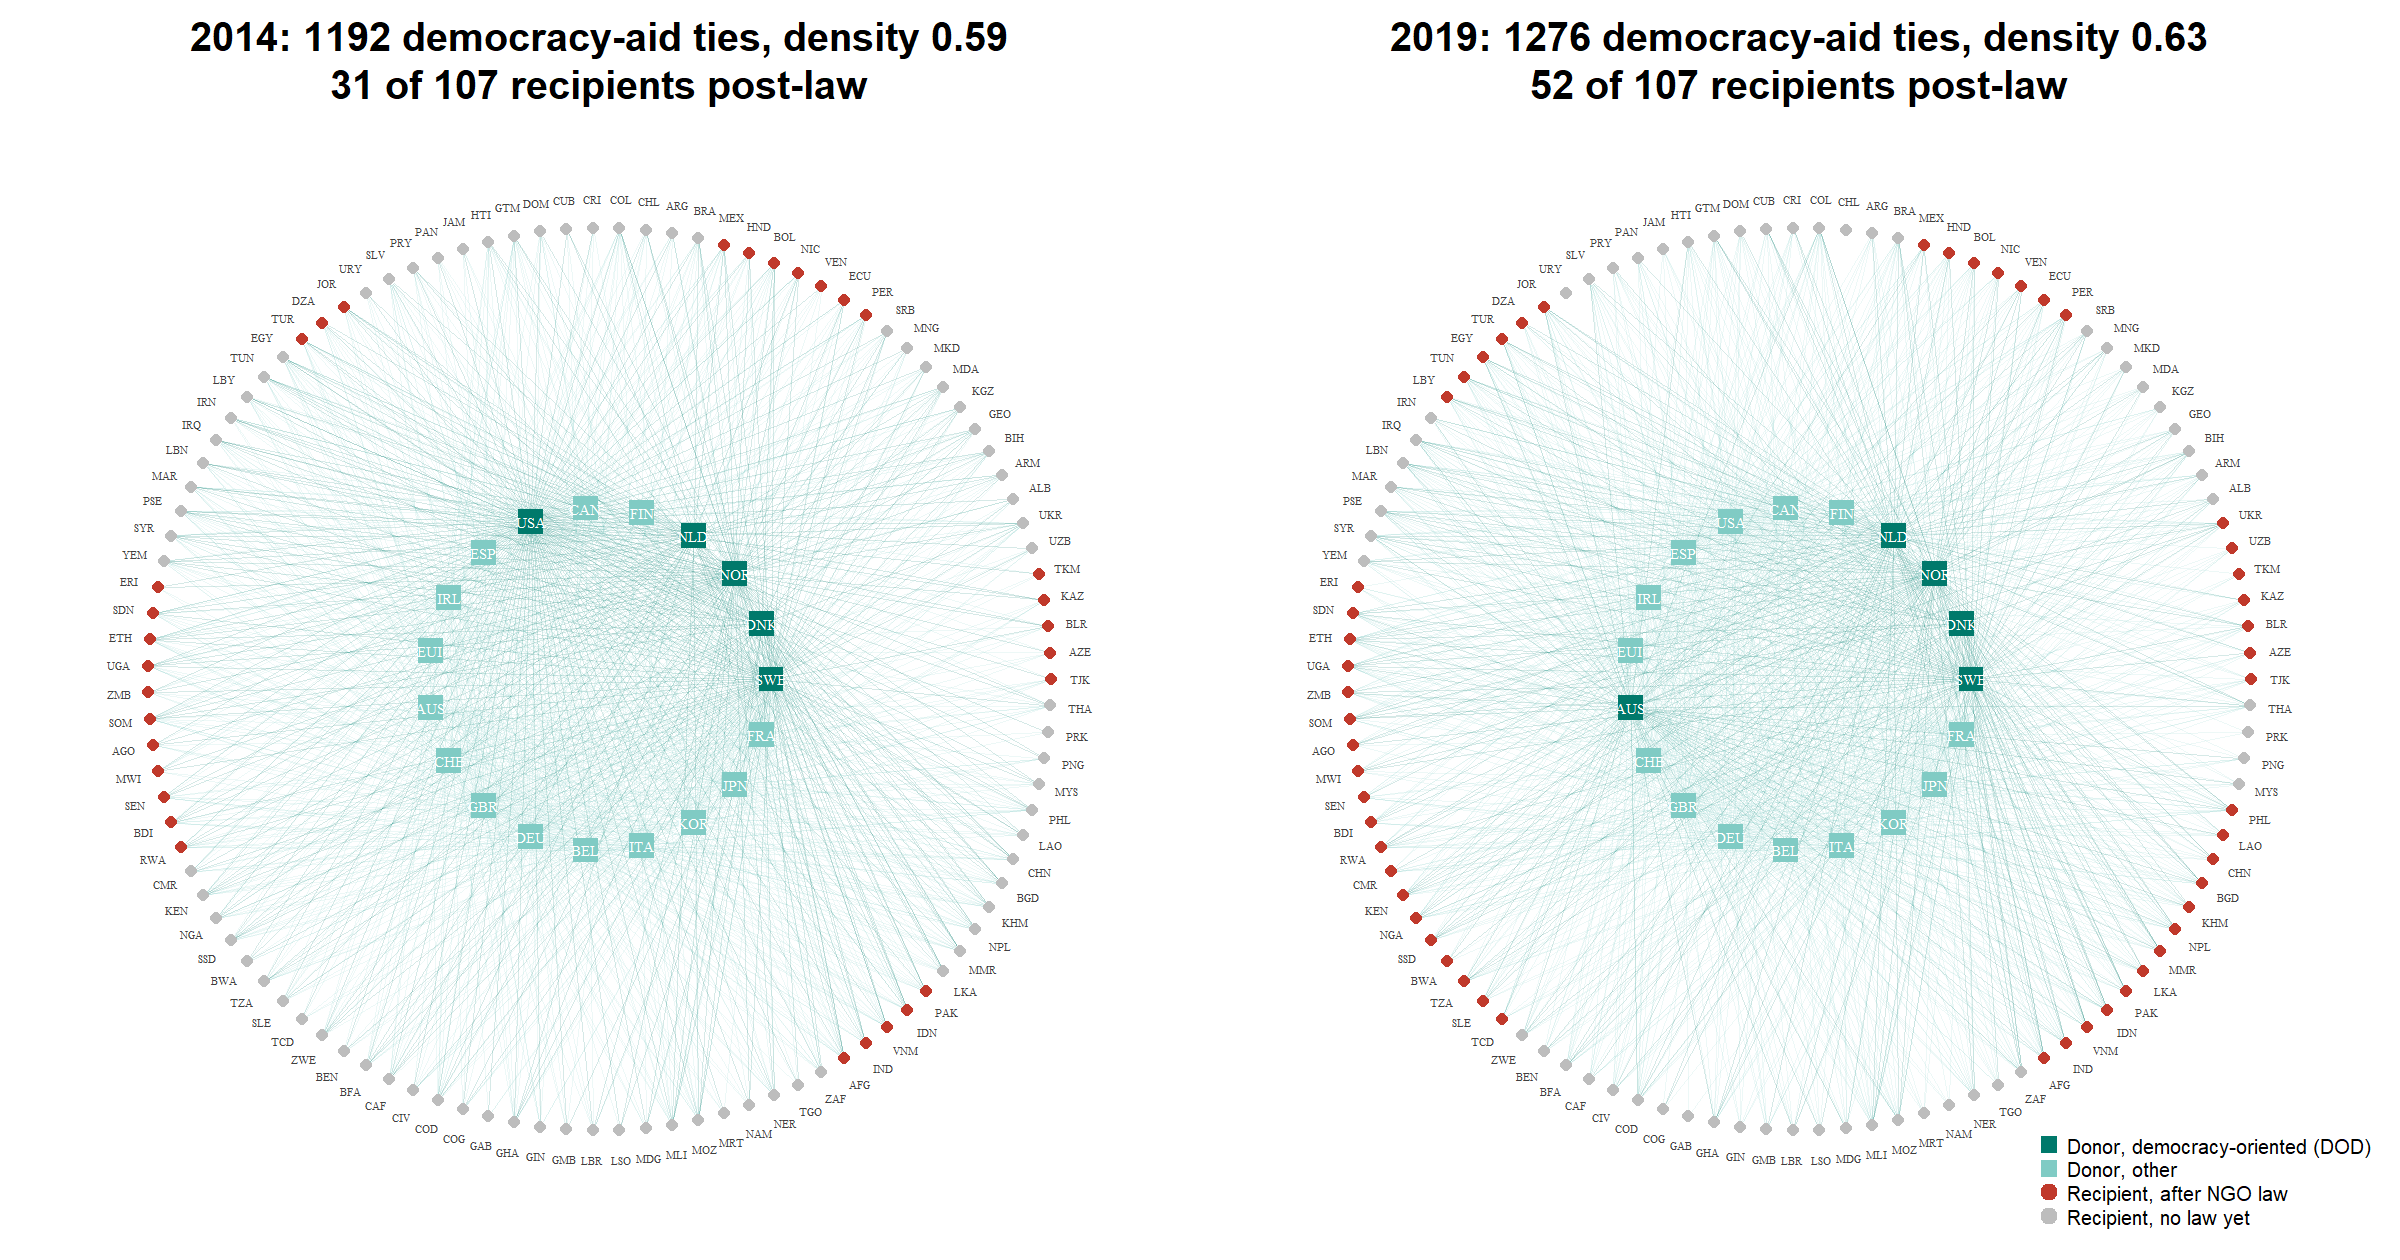
\includegraphics[width=\textwidth]{fig_N1_network_2014_2019.png}
  \caption{The democracy-aid network in 2014 and 2019, drawn with identical node positions.
  Squares are donors (inner ring, ordered by democracy-aid share; dark = democracy-oriented
  donor in that year, the paper's DOD measure). Circles are recipients (outer ring, grouped by
  region; orange = after its first restrictive NGO law). Edges are democracy-aid commitments.
  Source: \texttt{code/03\_network\_plot.R}.}
  \label{fig:net}
\end{figure}

\begin{figure}[H]
  \centering
  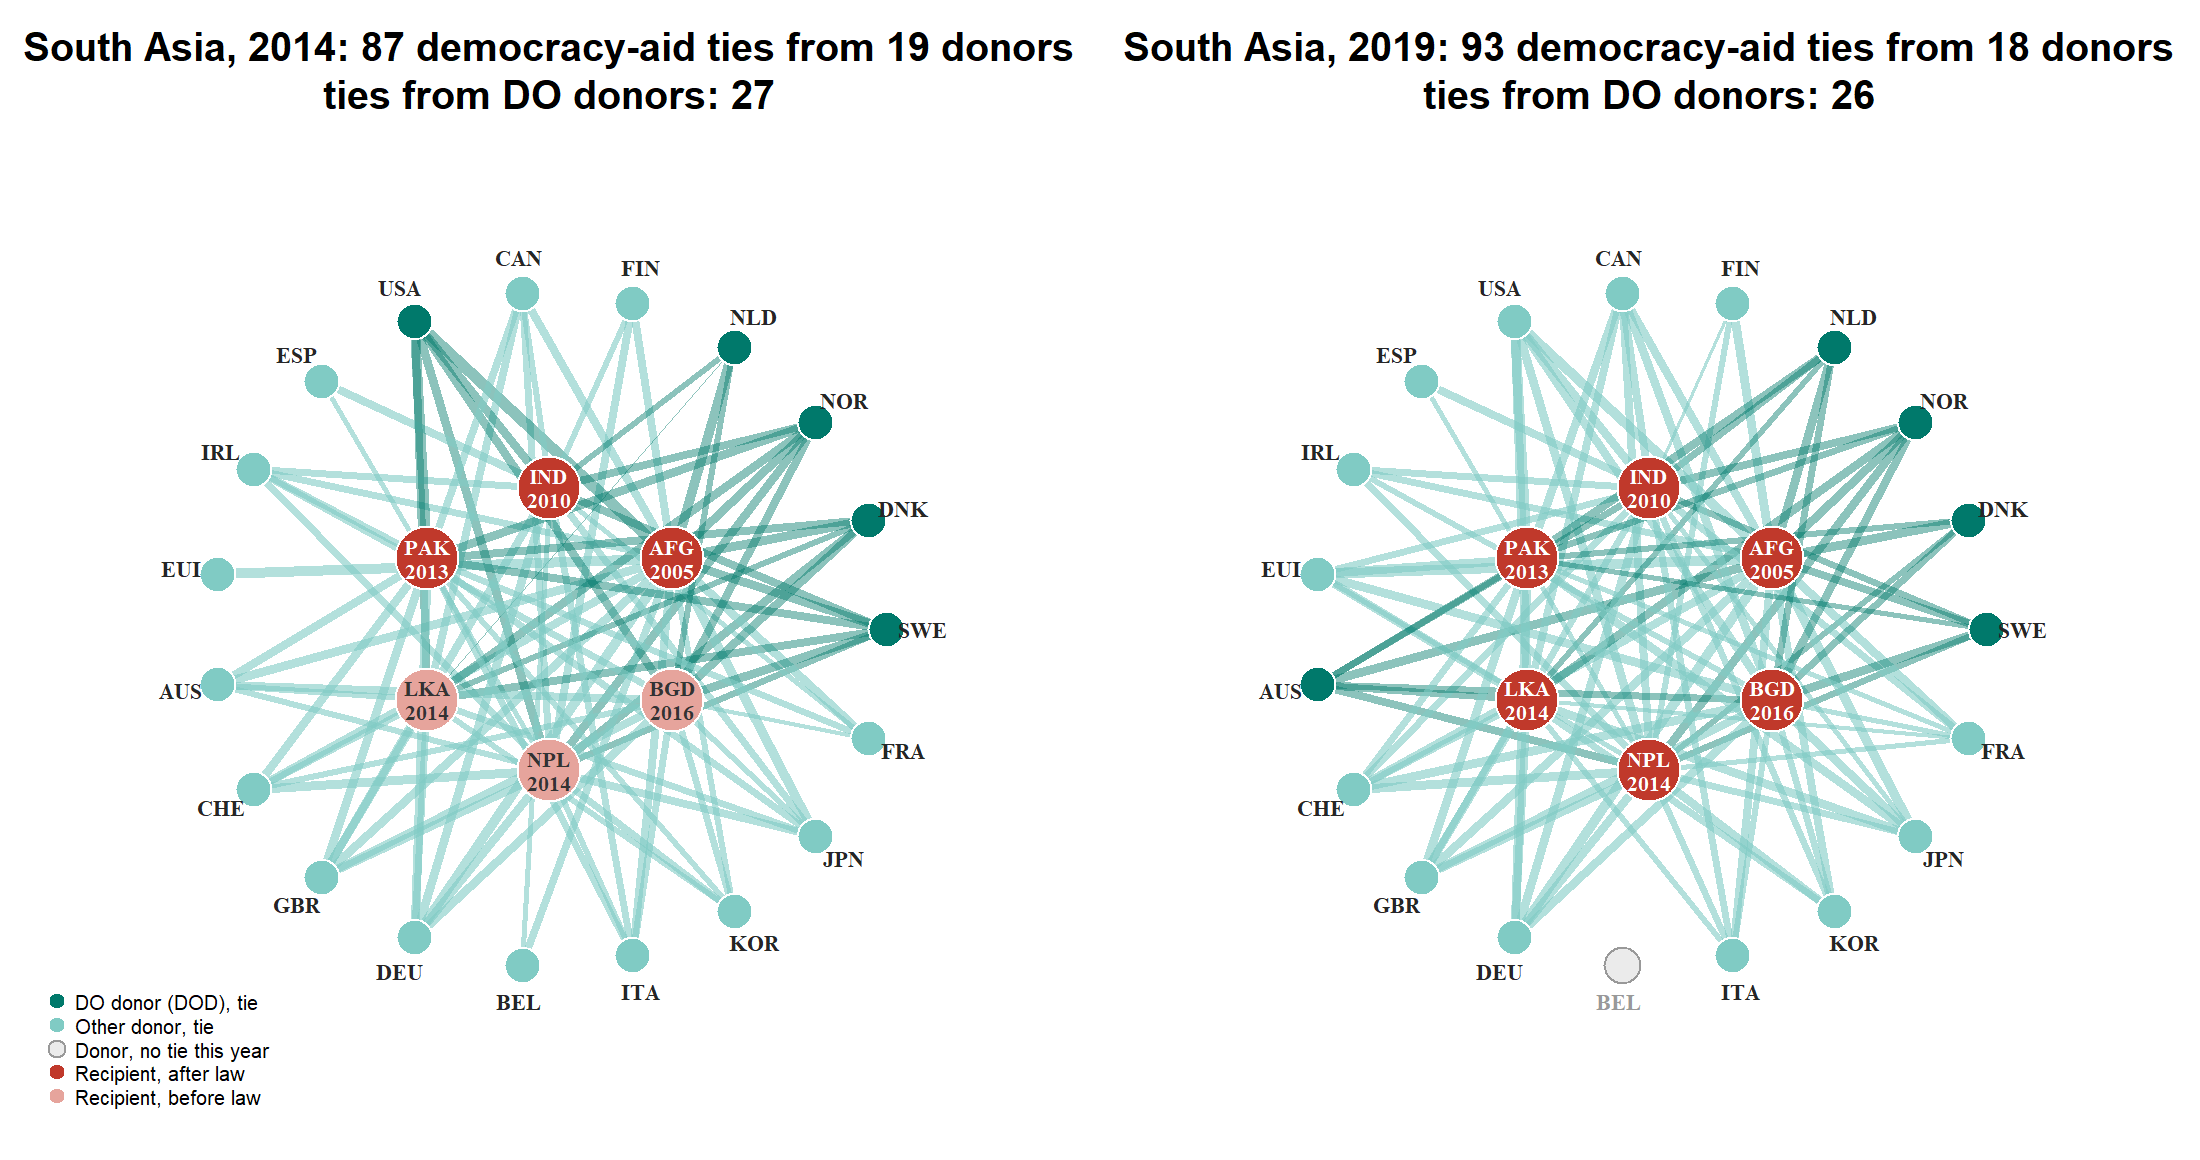
\includegraphics[width=\textwidth]{fig_N2_south_asia_2014_2019.png}
  \caption{South Asian sub-network, 2014 and 2019. Recipients are labelled with the year of
  their first restrictive NGO law; edge width is the logged commitment amount, on one scale for
  both years. Bhutan and the Maldives are excluded by the population rule.
  Source: \texttt{code/03\_network\_plot.R}.}
  \label{fig:sa}
\end{figure}

%===============================================================================
\section{Vertex Attributes}

Figures~\ref{fig:vdonor} and~\ref{fig:vrecip} show the distributions of the node attributes
used in the extension (\texttt{code/04\_vertex\_attributes.R}). Donors differ sharply in how
much of their aid goes to democracy and governance, which is the basis of the paper's
democracy-orientation measures. Recipients span the full range of regime types; 54 of them
pass a restrictive NGO law between 2005 and 2019, most of them after 2012.

\begin{figure}[H]
  \centering
  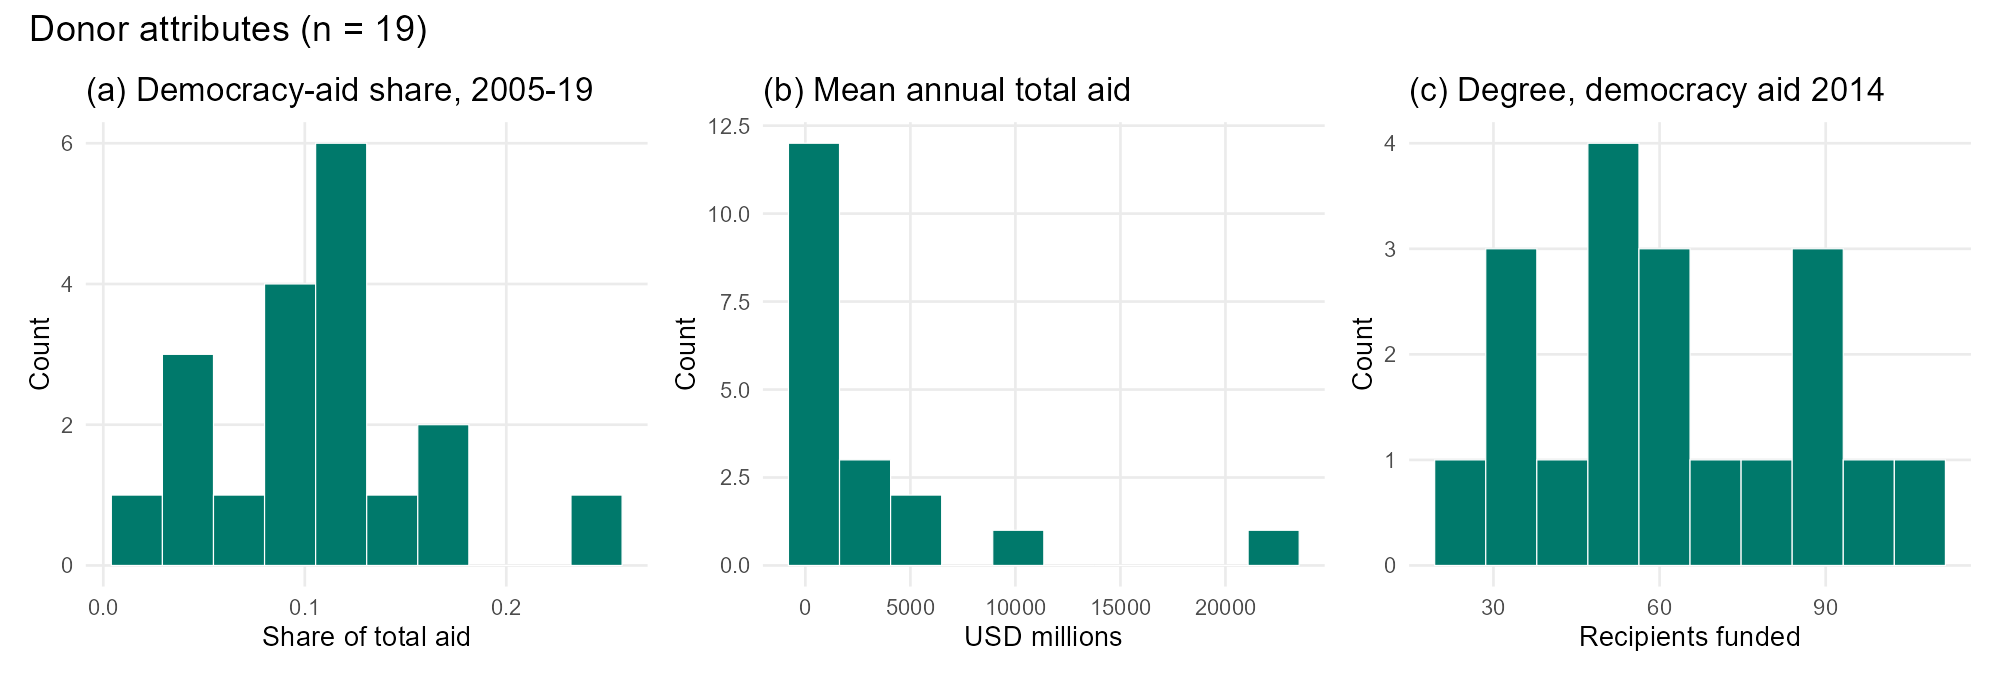
\includegraphics[width=\textwidth]{fig_V1_donor_attributes.png}
  \caption{Donor attributes ($n=19$): democracy-aid share of total aid (2005--2019), mean annual
  total commitments, and degree in the 2014 democracy-aid network.}
  \label{fig:vdonor}
\end{figure}

\begin{figure}[H]
  \centering
  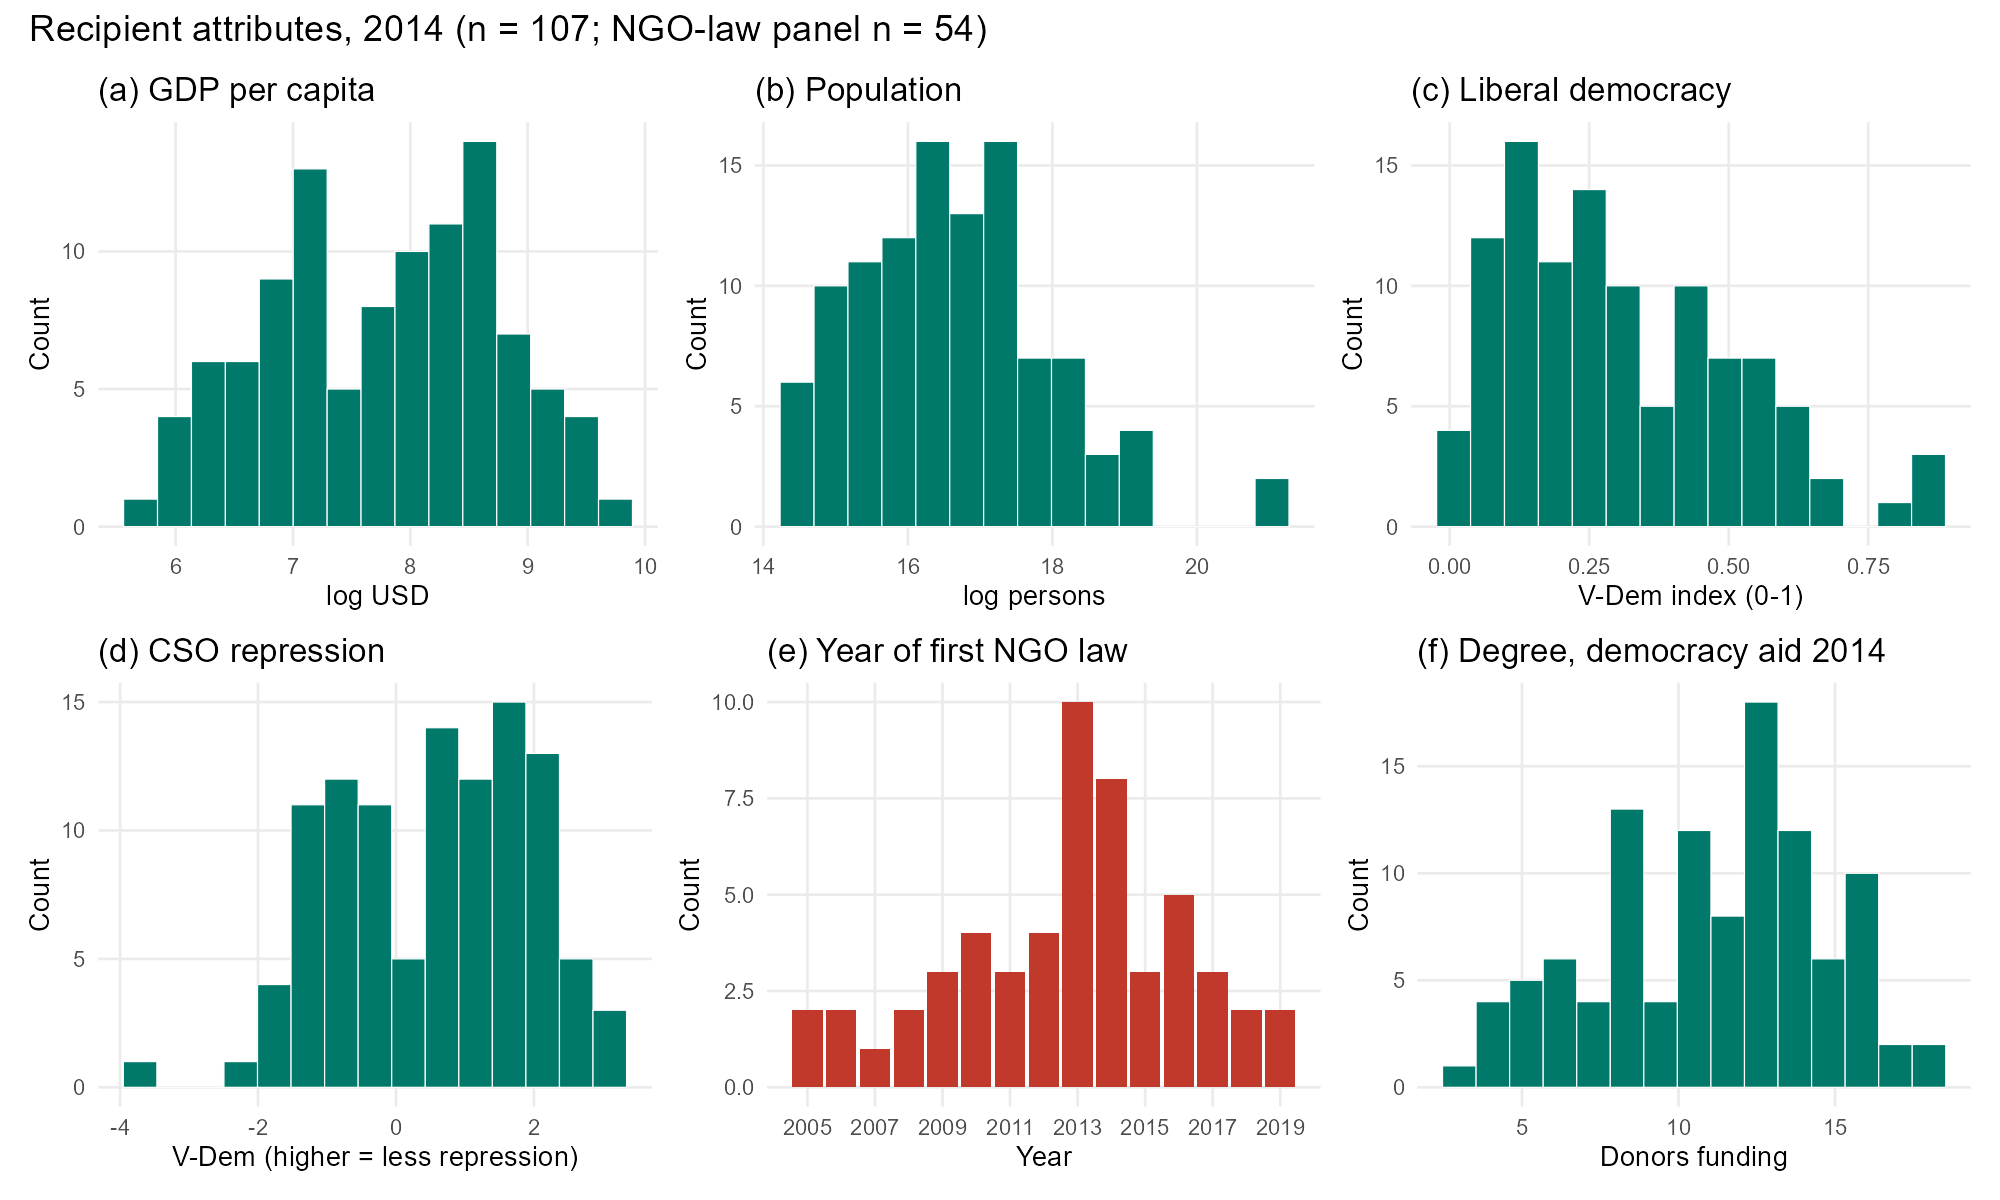
\includegraphics[width=\textwidth]{fig_V2_recipient_attributes.png}
  \caption{Recipient attributes in 2014: GDP per capita, population, V-Dem liberal democracy,
  V-Dem civil society repression, year of first restrictive NGO law (recipients that pass one),
  and degree in the 2014 democracy-aid network.}
  \label{fig:vrecip}
\end{figure}

%===============================================================================
\section{Reproduction of the Original Results}

\texttt{code/01\_replication.R} is the authors' replication script with relative paths and
optional sections. Every two-way fixed-effects table it produces (Tables 1 and 2 and appendix
Tables A3--A13 and the channel table, 14 in total) is identical, digit for digit, to the
authors' published output. The only exception is a labelling fix in Table A10: the original
code filled the year fixed-effects row for only three of the six columns, and the coefficients
are unchanged. Table~\ref{tab:event_response} and the table that follows it reproduce the
paper's Tables 1 and 2. Following the authors' instructions, the generalized synthetic control models are not
re-estimated (nine models with 1,000 bootstrap draws each). The figures are produced from the
authors' saved estimates (\texttt{gsc\_results.Rdata}, Dataverse). Figure~\ref{fig:gsc}
reproduces the paper's Figure 5.

\tab{tab_1_main_overall.tex}
\tab{tab_2_main_interaction.tex}

\begin{figure}[H]
  \centering
  \IfFileExists{../output/figures/fig_5a_dem_dod.jpg}{%
    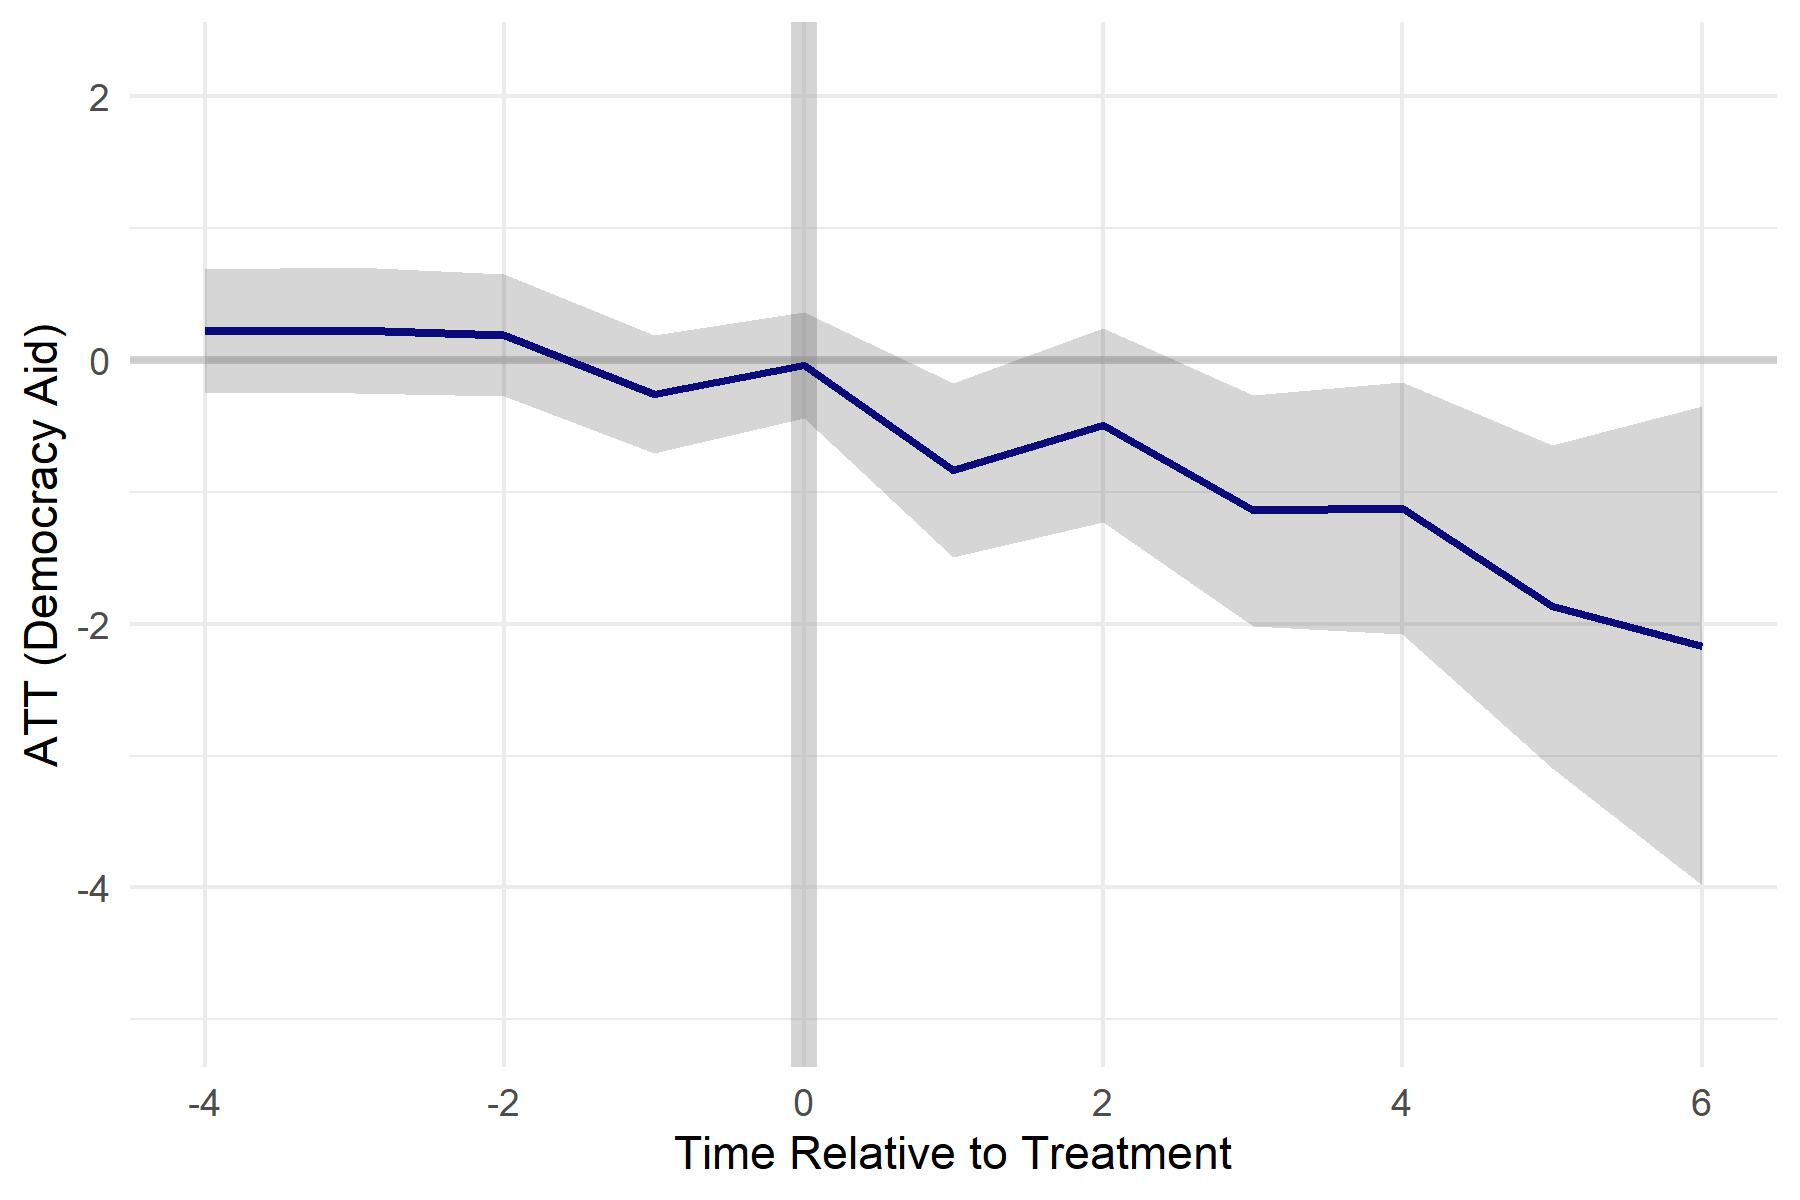
\includegraphics[width=0.48\textwidth]{fig_5a_dem_dod.jpg}\hfill
    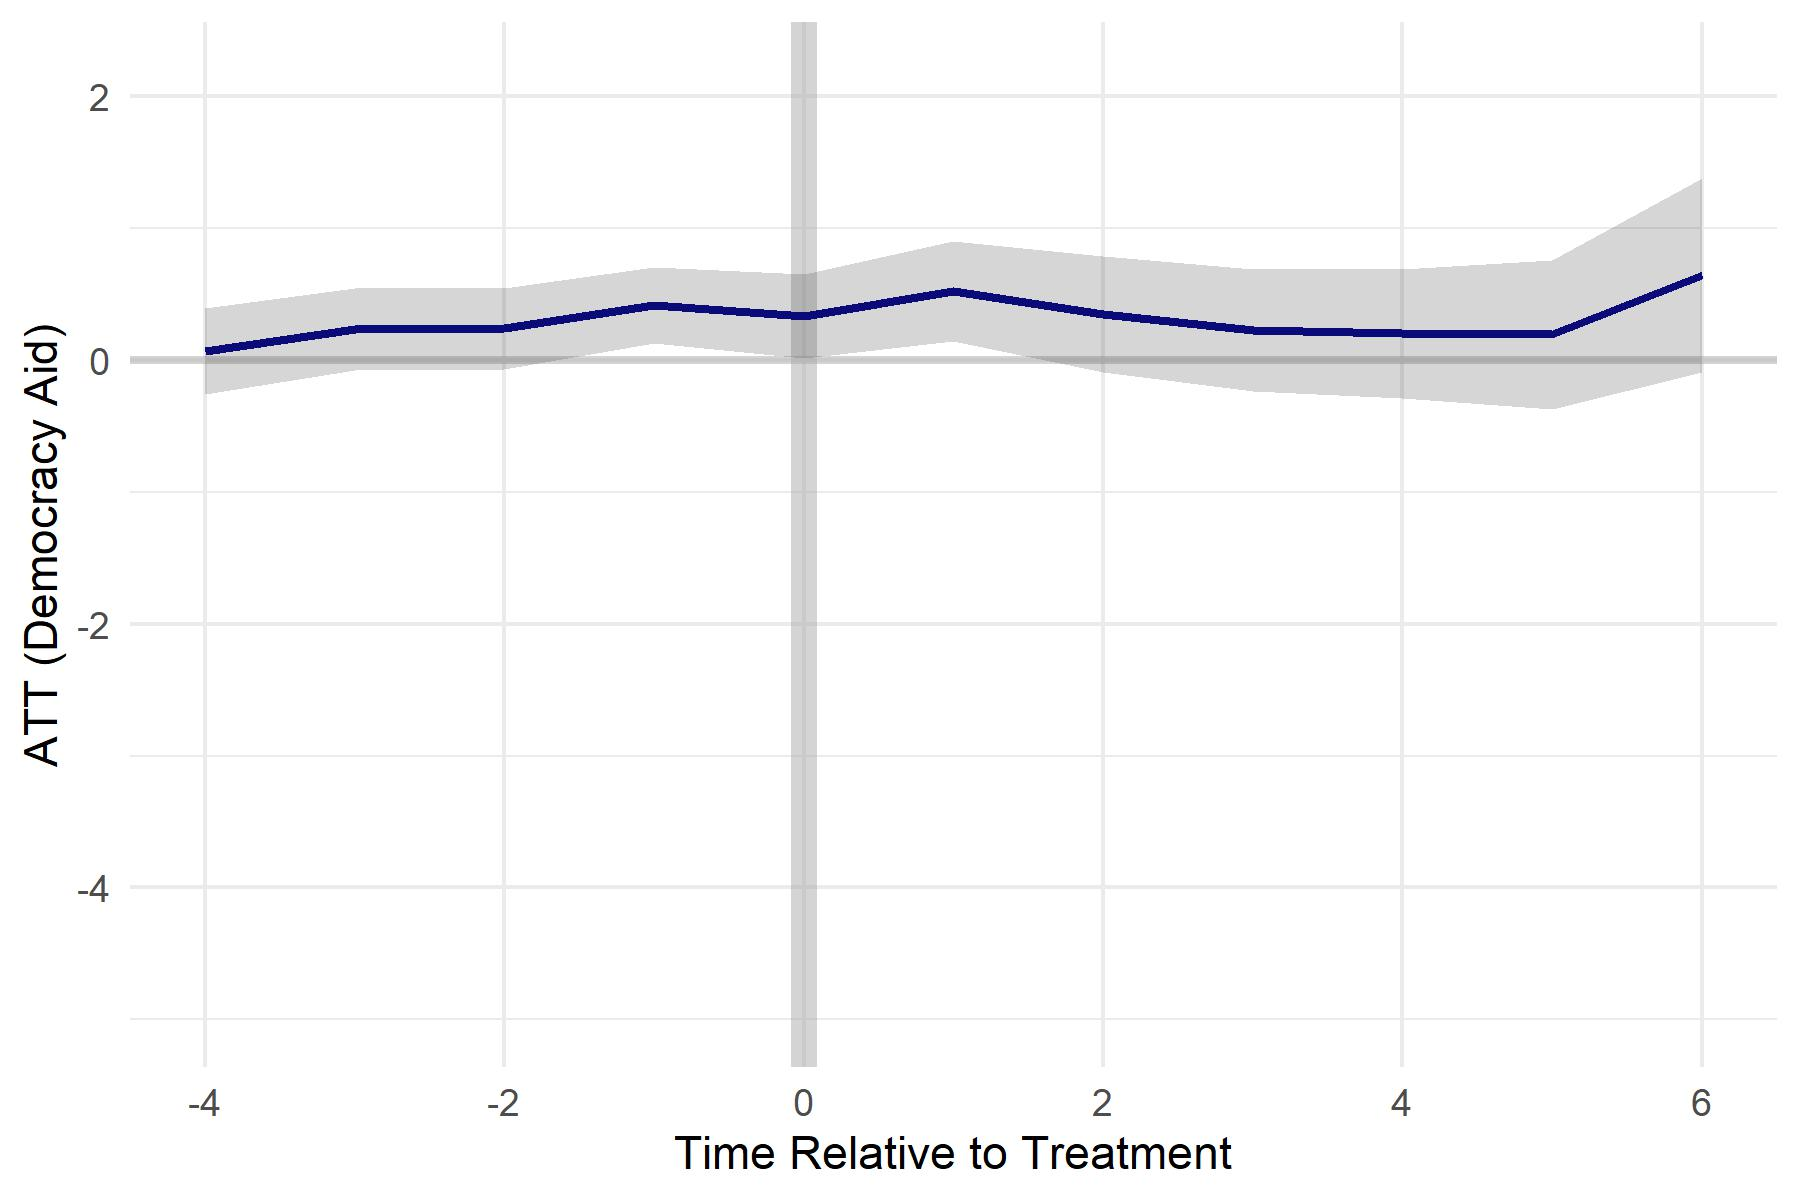
\includegraphics[width=0.48\textwidth]{fig_5b_dem_non.jpg}}{%
    \fbox{\parbox{0.9\textwidth}{\centering Run \texttt{code/01\_replication.R} with
    \texttt{data/gsc\_results.Rdata} present to generate this figure.}}}
  \caption{Effect of law passage on democracy aid, by donor orientation (generalized synthetic
  control); reproduces the paper's Figure 5. Left: democracy-oriented donors. Right: other donors.}
  \label{fig:gsc}
\end{figure}

\clearpage
\appendix
\section{Reproduced Robustness Tables}
All tables below are generated by \texttt{code/01\_replication.R} and match the published
appendix.

\tab{tab_A6_staggered_did.tex}
\tab{tab_A8_alternative_coding.tex}
\tab{tab_A9_continuous.tex}
\tab{tab_A10_drop_USA.tex}
\tab{tab_A11_nonzero.tex}
\tab{tab_A12_ihs.tex}
\tab{tab_A7_covariates.tex}
\tab{tab_A13_backsliding.tex}
\tab{tab_NR_channel.tex}

\bibliographystyle{apalike}
\bibliography{references}

\end{document}
